\chapter{Analysis}

\section{Introduction}

\subsection{Client Identification}
My client is John West, He is the manager of Waterbeach colts Football Clubs U16 team.  He has a high level of knowledge on computers, as he uses them on a daily basis within his job. He uses computers for a variety of tasks, ranging from basic to advanced. He mainly uses Windows systems however he has used a Mac in the past. John requires a team management program so that he can easily manage his team.
\subsection{Define the current system}
The current system is done with pen and paper. An Email system is used for contacting the players. The rest of the data that is required is all from memory.
\subsection{Describe the problems}
There is no tracking for who has replied to the emails and who hasn't, this is one problem.  Another is that most the data comes from the clients memory; this can be slow as it's easy to forget a certain item/criteria momentarily. Due to using pen and paper, the current system gets rather messy after a few team sheets are created. It is also prone to go missing. Paper waste is also high making it environmentally unfriendly.

\subsection{Section appendix}
What data or information is recorded in the current system?
-Nothing is physically recorded. I recall it all from memory.

What data or information is to be recorded in the proposed system? How much data will the proposed system record?
-The proposed system is going to hold Player and Match data. The Player data will 
include contact information as well as positions and match stats. The Match data will include results,fixtures,goals for/against etc.

How frequently will the data need to be updated?
-The data will need to be updated on a weekly basis(after a match is played) unless there is a change in player contact information then it will need to be updated more frequently. 

Will new records need to be added or old ones deleted? How often?
-New records will need to be added when a player joins the club, and records will need to be deleted when players leave. This shouldn't be very often.

Will the changes come in batches or in ones and twos?
-The changes should come in small batches as players can only join/leave in a certain period.

How important is the data or information that is recorded?
- The data is very important because without it the system wouldn't be helpful. 

What inputs are required for the proposed system?
-Initially all the data will be required. On a weekly basis only 'Who's available' will be required.

What are the outputs from the current system?
-A rough paper copy of the team sheet. 

What outputs will be required from the proposed system?
-A more detailed team sheet. That can be clearly read and understood.

Are hard copies required?
-Yes as I cant take my computer to games. 

How often will outputs be required?
-Outputs will be required on a weekly basis.

Is security an issues?
-The system will store personal data (contact information)

Should there be restricted access to particular areas?
-No

How are exceptions and errors handled in the current system?
-If an error occurs then i have to restart. 

Does the user have a particular solution in mind?
-I have an idea of what i want it to look like. 
\section{Investigation}

\subsection{The current system}
The current system is done with pen and paper. A computer is used for contacting the players. The client has to manually collect all the computer data and copy it down to paper. The rest of the data that is required is all from memory. Currently the client makes note of who is/isn't available on paper. He collects this data from email replies.  He then works out where players can play and sorts out a team sheet for the upcoming game.


\subsubsection{Algorithms}

func bubblesort( playerlist.rating)
    for each from 1 to len(playerlist)
        for each from 0 to N - 1
           if playerlist.each.rating > playerlist.each[+1].rating
              swap( playerlist[each], playerlist[each + 1] )
end func
For each in playerlist:
	if playerlist.each.position = (Required positon)\:
		team\_sheet.append(playerlist.each)
		playerlist.pop(each)
		Each -> len.(playerlist)
		
	
End For
The for loop would be run for every position.

Substitutes ->  playerlist 

\subsubsection{Input Forms, Output Forms, Report Formats}
\begin{figure}[H]
	This is what the current system looks like, pen and paper form, the system should have a similar layout.
	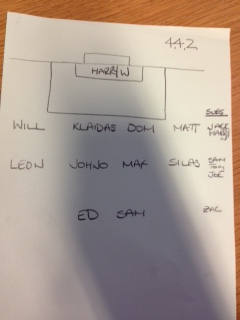
\includegraphics{formation}
	
	
	This is the available squad list, this is where the client currently chooses the team from. 

	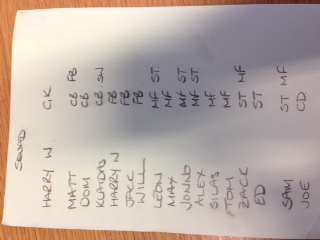
\includegraphics{squad}
\end{figure}

\subsection{The proposed system}
Proposed system is going to set out the team sheet, show injuries and possible replacements. It will also store all the information of players with attributes and contact information along with data from previous games. It should also include an email reply system to show who's available for upcoming events. New records will need to be added every time a new player joins and a record will need to be deleted every time a player leaves the club.

\subsubsection{Data sources and destinations}
\begin{table}[H]
\centering

\label{my-label}
\begin{tabular}{|l|l|l|l|}
\hline
Source               & Data             & Example Data    & Destination \\ \hline
Player Input         & Player Forename  & Harry           & Form        \\ \hline
Player Input         & Player Surname   & West            & Form        \\ \hline
Player Input         & Player Email     & Hwest@gmail.com & Form        \\ \hline
Player Input         & Player Position  & GK              & Form        \\ \hline
Client/manager Input & Player Rating    & 8               & Form        \\ \hline
Client Input         & Form             &                 & System      \\ \hline
Client Input         & PlayerInjured    & N               &             \\ \hline
System               & {\ul Player ID}  & 123             & System      \\ \hline
System               & {\ul Match ID}   & 987             & System      \\ \hline
Client Input         & Match Result     & W               & System      \\ \hline
Client Input         & Match Opposition & Milton          & System      \\ \hline
Client Input         & Goal Quantity    & 2               & System      \\ \hline
\end{tabular}
\end{table}

\subsubsection{Data flow diagrams}
\begin{figure}[H]
	\includegraphics{dataflow}
\end{figure}

\subsubsection{Data dictionary}

\begin{table}[H]
\centering
\label{my-label}
\begin{tabular}{|p{2.5cm}|p{1cm}|p{1.5cm}|p{2.5cm}|p{2.5cm}|p{2.5cm}|} 
\hline
Name            & Data Type & Length   & Validation                    & Example Data    & Comment                        \\ \hline
PlayerID        & Integer   & 3 Digits & 3 Digits, Must exist          & 123             & Unique to each player          \\ \hline
PlayerForename  & String    & 15 Chars & Minimum of 3 digits           & Harry           & First name, capital first char \\ \hline
PlayerSurname   & String    & 20 Chars & Minimum of 3 digits           & West            & Surname, capital first char    \\ \hline
PlayerPosition  & String    & 2 Chars  & Must be 2 chars               & GK              & In caps                        \\ \hline
PlayerRating    & Integer   & 2 Digits & Maximum of 2 digits           & 8               & Most likely to only be 1 digit \\ \hline
PlayerEmail     & String    & 50 Chars & Must have an @                & Hwest@gmail.com & Contact for the player         \\ \hline
MatchID         & Integer   & 3 Digits & 3 digits, must exist          & 869             & Unique to match                \\ \hline
MatchDate       & String    & 8 Chars  & Must exist                    & 23/09/14        & Date of the match              \\ \hline
MatchResult     & String    & 1 Chars  & Must exist                    & W               & W=Win, L=lose, D=Draw          \\ \hline
MatchOpposition & String    & 20 Chars & Minimum of 3 digits           & Milton          & Opposition name                \\ \hline
GoalQuantity    & Integer   & 2 Digits & At least one digit must exist & 2               & 99\% will only be one digit    \\ \hline
\end{tabular}
\end{table}

\subsubsection{volumetrics}
The system should be able to store 16 players and their data initially and cater for expansion to 30 players and their data. It will also need to cater for 40 games initially with the ability to expand to 400(10 seasons). 
\section{Objectives}

\subsection{General Objectives}
To create an easy to use team sheet selector.
\subsection{Specific Objectives}
To allow the client to edit player details and add game details on a weekly basis.
\subsection{Core Objectives}
The system must lay out a team sheet. It must also show the availability of players, this may be due to injuries or just being away on that date.     
\subsection{Other Objectives}
It would be desirable to have individual stats for each player rather than an overall rating giving a more detailed overview of a players ability.
\section{ER Diagrams and Descriptions}

\subsection{ER Diagram}
\begin{figure}[H]
	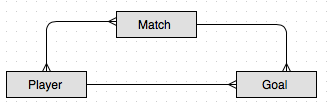
\includegraphics{ER}
\end{figure}

\subsection{Entity Descriptions}
Player( {\ul PlayerID},PlayerForename,PlayerSurname,PlayerRating,PlayerEmail,PlayerPosition,PlayerAvailable)
Match({\ul MatchID},MatchDate,MatchResult,MatchOpposition)
Goals(MatchID,PlayerID,GoalQuantity)
\section{Object Analysis}

\subsection{Object Listing}
 My objects are Players, Goals and Matches. 
\subsection{Relationship diagrams}
\begin{figure}[H]
	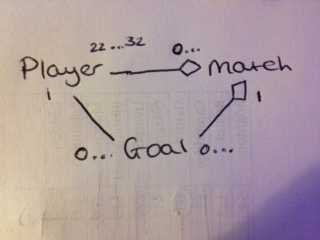
\includegraphics{classdiagram}
\end{figure}

\subsection{Class definitions}
\begin{figure}[H]
	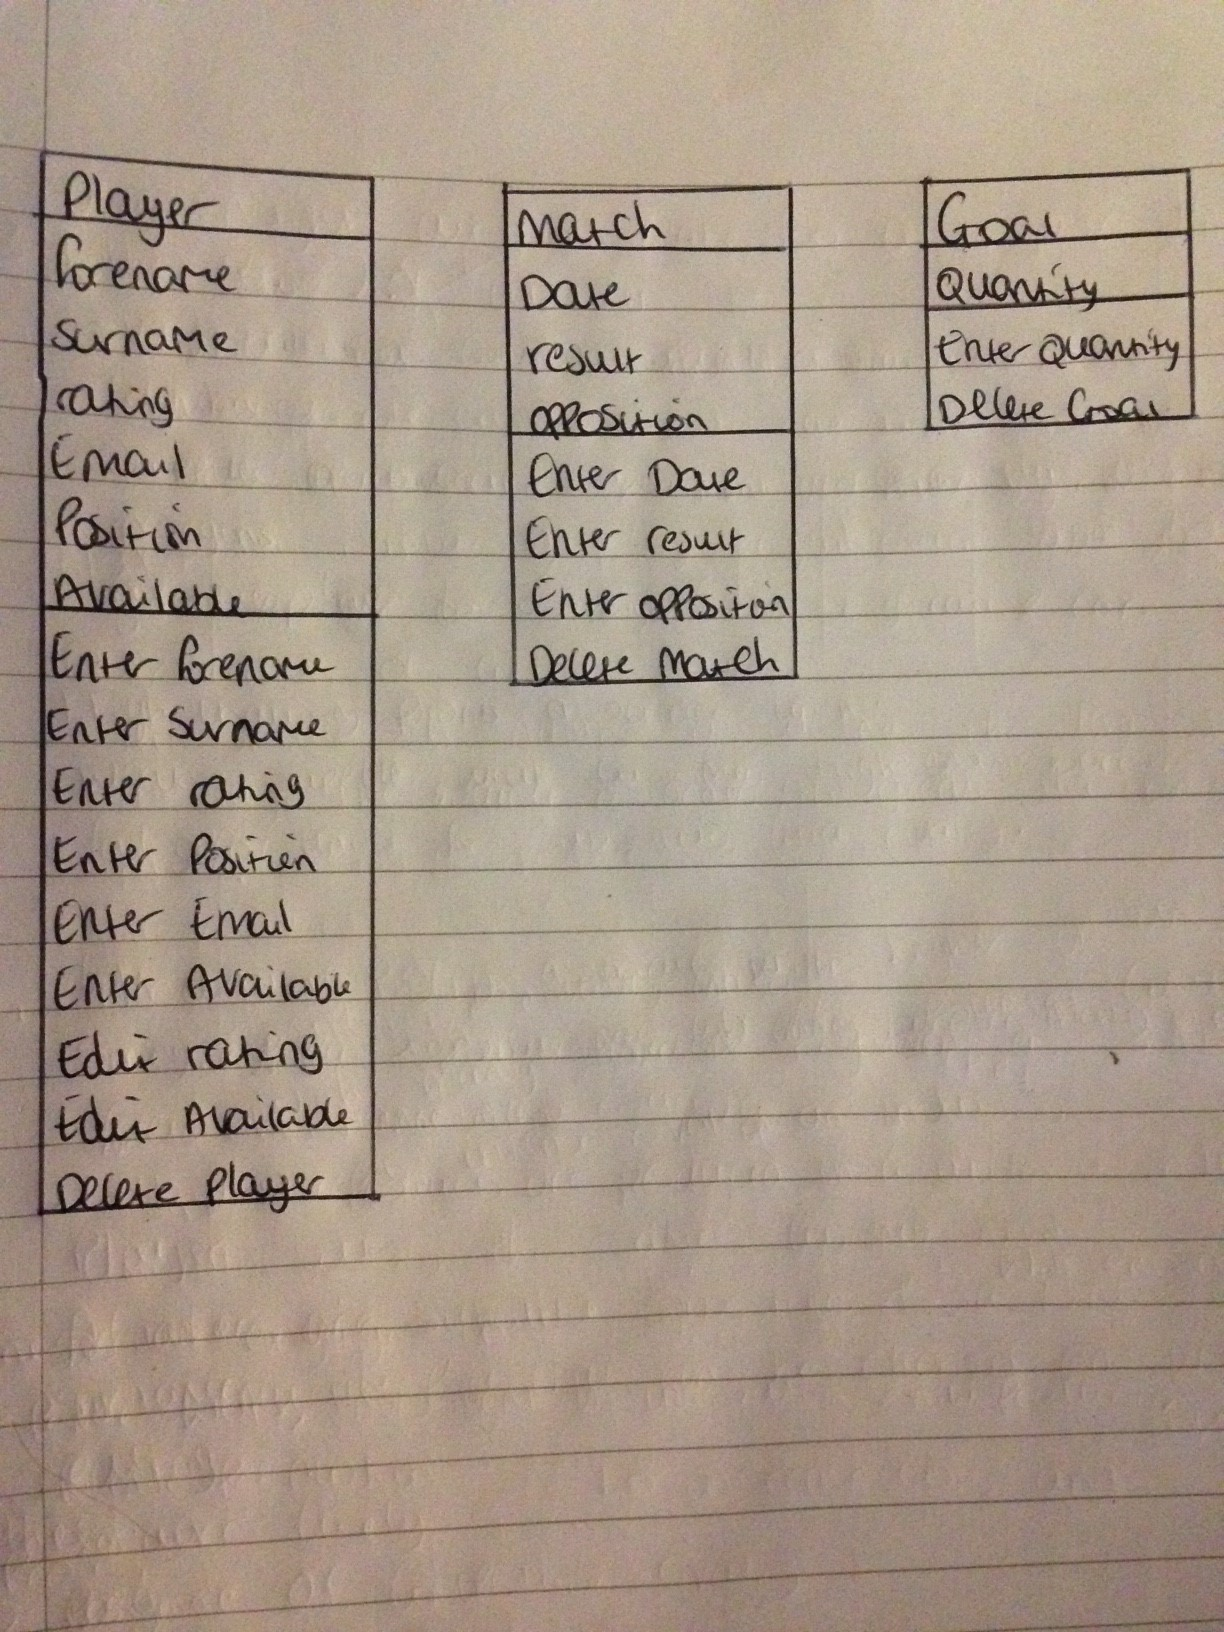
\includegraphics[width=150mm]{classdef}
\end{figure}


\section{Constraints}

\subsection{Hardware}
The client has a windows desktop PC and laptop along with an Ipad so is use to a couple of operating systems. The program would most likely be run on a Windows PC however using the portability of the Ipad would be advantageous.
\subsection{Software}
The client has no preferences on the software that is used and has therefore left it up to me to choose.  
\subsection{Time}
The client would like the program ready before June 2015, this would give the client time to become familiar with the program and fix any bugs that may occur. 
\subsection{User Knowledge}
The user's job heavily involves computers, this gives him good background knowledge on how they operate. On a daily basis he completes basic and complex task demonstrating his depth of knowledge. 
\subsection{Access restrictions}
Anybody will be able to access the current team sheet as it is useful for the players to see who they are playing with and what position they are playing. Due to the system containing contact information there will need to be restricted access on some areas of program to ensure that personal information is not shared.   

\section{Limitations}

\subsection{Areas which will not be included in computerisation}
All areas relevant to the client and his team are going to be computerised.
\subsection{Areas considered for future computerisation}
The league table could be considered for future computerisation, along with other teams player statistics.
\section{Solutions}
My system could use a pre made database, this will benefit me and the client because it will save time compared to writing a database. This means that the final deadline can be moved forward giving the client more time to learn the program.  However a pre made database wont be tailored to the clients needs and therefore will have unnecessary extras. A high quality pre made database may also need to be bought. This will cost the client. Writing my own database for the project will benefit the client because the database will be tailored to there exact needs however it will be much more time consuming, writing and debugging, than a pre made database.

Another option for the system is whether to have it as a desktop application or a web application. Having it as a desktop application will allow portability as the client doesn't need to be connected to the internet to be able to use the system (offline use). Having portability will be very useful for my client as it means that they can use the system at the pitch side on an Ipad. Depending on internet connection, the desktop application is going to run quicker. However making the system an web app will mean that it is easily accessible all the players. This means that they can look up who's on the team sheet for the upcoming game. A web app will require a web database, poor internet connection will jeopardise this link and therefore cause the system to crash. This wont happen on a desktop app. 
\subsection{Alternative solutions}

\subsection{Justification of chosen solution}
I have chosen to write my own database for the client as it will then be tailored to there exact needs, improving efficiency due to no added extras. I have also chosen to make the system a desktop application as the portability aspect will be very useful.